\chapter*{Введение}
\addcontentsline{toc}{chapter}{Введение}

Настоящее учебное пособие предназначено для~изучения правильной организации и~проведения технического обслуживания легких многоцелевых гусеничных транспортеров-тягачей МТЛБ. 

Техническое обслуживание транспортера-тягача (рис.~\ref{mtlb1}) включает следующие виды: 

\begin{itemize}

    \item контрольный осмотр перед выходом из~парка; 
    \item контрольный осмотр в~пути (на~привалах и~остановках); 
    \item ежедневное техническое обслуживание; 
    \item техническое обслуживание №1 (ТО-1) через \range{800}{1000}~км пробега;
    \item техническое обслуживание №2 (ТО-2) через \range{2400}{3000}~км пробега;

\end{itemize}

\begin{figure}[]
    \centering
    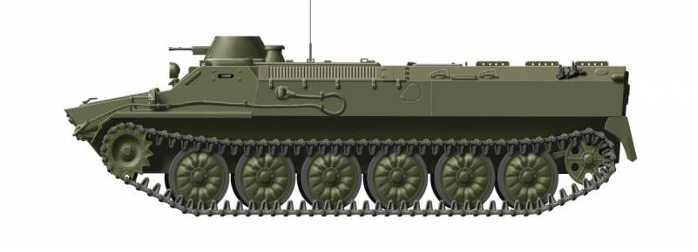
\includegraphics[width=\textwidth]{src/mtlb_1.png}
    \caption{Транспортер-тягач МТ-ЛБ}
    \label{mtlb1}
\end{figure}

Кроме контрольных осмотров и~технических обслуживании  №1 и~2 проводятся дополнительные работы по~уходу и~сбережению транспортеров-тягачей: 

\begin{itemize}
    \item один раз в~месяц в~парковые дни;
    \item при~переводе транспортеров-тягачей на~сезонную эксплуатацию;
    \item при~содержании транспортеров-тягачей в~консервации.
\end{itemize}

В~пособие предусмотрены дополнительные операции по~техническому обслуживанию при~эксплуатации транспортеров-тягачей в~районах Крайнего Севера, в~пустынно-песчаных и~горных районах, а~также в~период распутицы.


Учебное пособие содержит:
\begin{itemize}
    \item перечень операций по~каждому виду осмотра и~технического обслуживания; 
    \item указания о~составе исполнителей, объеме трудовых затрат и~времени простоя транспортеров-тягачей при~проведении осмотров и~обслуживании;
    \item перечень операций по~консервации транспортеров-тягачей и~техническому обслуживанию их в~консервации; 
    \item технологические карты на~наиболее сложные операции по~техническому обслуживанию.
\end{itemize}

В~табл.~\ref{worktime} и \ref{worktime2} даны трудовые затраты и~время простоя транспортеров-тягачей при~контрольных осмотрах и~техническом обслуживании. 

Верхние пределы трудозатрат и~времени простоя относятся к~выполнению технического обслуживания с~полным объемом регулировочных работ, в~знаменателе~--- то~же, но~при~эксплуатации транспортеров-тягачей в~тяжелых дорожных условиях (периоды весенней и~осенней распутицы, работы после форсирования водных преград). 


\begin{sidewaystable}
    \footnotesize
    {
    \newcommand{\length}{1.97cm}
    \newcommand{\longlength}{5cm}
    \centering
    \begin{tabular}{|m{\longlength}|>{\tc}m{\length}|>{\tc}m{\length}|>{\tc}m{\length}|>{\tc}m{\length}|>{\tc}m{\length}|}
        \hline
        \multirow{2}{\longlength}{\centering Вид работ} & \multicolumn{5}{c|}{\textbf{Трудозатраты, \textit{чел.-час}}} \\ 
        \cline{2-6}
        & \textbf{механика-водителя} & \textbf{механика} & \textbf{электрика} & \textbf{слесаря} & \textbf{общие} \\
        \hline
        Контрольный осмотр перед выходом из~парка & 27--40~мин &~--- &~--- &~--- & 27--40~мин  \\
        \hline
        Контрольный осмотр в~пути & 20--30~мин &~--- &~--- &~--- & 27--40~мин  \\
        \hline
        Ежедневное техническое обслуживание & 
            \begin{tabular}{c}
                 1,2--2,3 \\
                 \hline
                 1,6--2,7
            \end{tabular} &~--- &~--- &~--- & 
            \begin{tabular}{c}
                 1,2--2,3 \\
                 \hline
                 1,6--2,7
            \end{tabular}
            \\
        \hline
        Техническое обслуживание №1 &
            \begin{tabular}{c}
                 3,8--9,1 \\
                 \hline
                 4,7--9,4
            \end{tabular} &
            \begin{tabular}{c}
                 1,2--1,6 \\
                 \hline
                 2,1--2,4
            \end{tabular} &
            \begin{tabular}{c}
                 0,5--0,7 \\
                 \hline
                 1,9--2,2
            \end{tabular} &
            \begin{tabular}{c}
                 1,5--1,7 \\
                 \hline
                 1,9--1,2
            \end{tabular} &
            \begin{tabular}{c}
                 7--13,1 \\
                 \hline
                 9,6--15
            \end{tabular} \\
        \hline
        Техническое обслуживание №2 &
            \begin{tabular}{c}
                 10,2--17,1 \\
                 \hline
                 12,7--17,6
            \end{tabular} &
            \begin{tabular}{c}
                 4--5 \\
                 \hline
                 4,6--5,8
            \end{tabular} &
            \begin{tabular}{c}
                 1,2--1,7 \\
                 \hline
                 2--3
            \end{tabular} &
            \begin{tabular}{c}
                 2,9--3,9 \\
                 \hline
                 3,7--4,8
            \end{tabular} &
            \begin{tabular}{c}
                 18,3--28,3 \\
                 \hline
                 23--31,2
            \end{tabular} \\
        \hline
        Подготовка к~летнему периоду эксплуатации (дополнительно к~ТО-1 и~ТО-2) & \range{2}{2,2} &~--- & 0,5 & 1 & \range{3,5}{3,7} \\
        \hline
        Подготовка к~зимнему периоду эксплуатации (дополнительно к~ТО-1 и~ТО-2) & \range{4,6}{4,9} & 0,5 & 0,5 & 2,1 & \range{7,7}{8} \\
        \hline
    \end{tabular}
    \caption{Трудозатраты на~контрольные осмотры и~техническое обслуживание}
    \label{worktime}
    }
    \textit{Примечания:} 
    \begin{itemize}
        \item \textit{В~трудозатраты на~контрольный осмотр перед выходом из~парка не~включено время на~пуск и~прогрев двигателя при~низких температурах воздуха.} 
        \item \textit{Трудоемкость работ по~ежедневному обслуживанию приведена без~учета времени на~уборочно-моечные работы, которое для~транспортеров-тягачей различной загрязненности составляет \range{1,5}{3}~чел.-час.} 
    \end{itemize}
\end{sidewaystable}

\begin{table}
    \newcommand{\length}{1.82cm}
    \centering
    \begin{tabular}{|m{\length}|m{\length}|m{\length}|m{\length}|m{\length}|}
        \hline
        \multirow{2}{\length}{\tc ЕТО} & \multirow{2}{\length}{\tc ТО-1}  & \multirow{2}{\length}{\tc ТО-2} & \multicolumn{2}{m{\dimexpr \length * 2 + 12pt \relax}|}{\tc Подготовка к~периоду эксплуатации} \\ 
        \cline{4-5}
        &&& \tc летнему & \tc зимнему \\
        \hline
        \tc \range{1,2}{2,7} & \tc\range{3,8}{9,4} & \tc\range{10,2}{17,6} & \tc 3,7 & \tc 8 \\ 
        \hline
    \end{tabular}
    \caption{Простой транспортера-тягача при~техническом обслуживании и~при~подготовке его к~эксплуатации в~летний и~зимний периоды, \textit{ч}}
    \label{worktime2}
\end{table}

При~определении времени на~техническое обслуживание заместитель командира по~технической части (начальник автотракторной службы) должен учитывать техническое состояние и~потребность в~проведении регулировок тех или~иных агрегатов и~механизмов транспортеров-тягачей. 


